\documentclass{article}

\usepackage{fullpage}  % Makes the text margins smaller
\usepackage{graphicx} % To include figures
\usepackage{fancyvrb} % Includes the \VerbatimInput command to read in code files
\usepackage{amsmath}
\DeclareGraphicsExtensions{.png}
\renewcommand*{\arraystretch}{2}

\author{Cody Lieu, Yixin Lin}
\title{COMPSCI 527 Homework 6}

\begin{document}
\maketitle

% How to include pictures with captions
% 
% \begin{figure}[h!]
%   \caption{caption}
%   \centering
% 	\includegraphics{filename}
% \end{figure}


\section{Introduction}

3D object reconstruction from a set of 2D images is fundamentally an ill-conditioned problem, due to its inverse nature. We investigate the effects of noise and other parameters on the success of reconstructing the original 3D object from stereo images. To this effect, we use the 8-point algorithm with the Hartley preprocessing\cite{hartley} (by using the canonical homogeneous coordinates). We quantify the accuracy of the reconstructed 3D object by measuring three types of errors: motion, structure, and reprojection error.

Our goal in this paper is to investigate the following questions:
\begin{itemize}
\item Which types of error fail first when enough noise is added for the shape to be unrecognizable? 
\item What happens when we change the image resolution but keep sigma fixed?
\end{itemize}

\section{Progression of failure with increasing levels of noise}

% Explanation of problem
\subsection{Introduction}

The software provided creates a simulated world with a square object (with multiple colored squares on each side) and two cameras, adds Gaussian noise to the image coordinates, and runs the eight-point algorithm for 3-d reconstruction. Because reconstruction is a ill-conditioned/ill-posed problem (due to its inverse nature), small errors in the data will often result in large errors in the 3D reconstruction. 

We investigate the effect of pseudo-random Gaussian noise on different types of errors, especially as the image become so distorted that the reconstructed shape becomes unrecognizable.

We have three broad categories of errors:

\begin{enumerate}
  \item Motion error: the difference between true and computed motion, for both translation and rotation, measured in degrees
  \item Structure error: the difference between true and computed structure, measured in RMS average percentage error of the overall size of the object
  \item Reprojection error: the difference between the image of the original object and reprojected image of the reconstructed object, measured in RMS pixels per point
\end{enumerate} 

We pose the question: at the point where enough noise has been added so that the reconstructed object is unrecognizable, what types of errors fail first?

% Hypothesis

% \subsection{Hypothesis}

% Experiment ran

\subsection{Methods}

The experiment we ran was to run the following procedure, in which a subroutine was applied on a range of sigmas from \texttt{0:.25:5}, with n = 150 for each sigma; we recorded the average errors for each, as shown in Figures 1-3.

\subsection*{Procedure}



\begin{enumerate}
  \item Create a 3D world, with object (Gaussian noise sigma = 0), two cameras, and the resulting images
  \item Compute the true transformation between the camera reference frames
  \item Compute the true structure
  \item Subroutine for each sigma in range \texttt{0:.25:4}
  \begin{itemize}
  	\item Add noise to the original image with sigma
  	\item Compute the resulting transformation figure
  	\item Measure and record motion, structure, and reprojection errors
  \end{itemize}
\end{enumerate} 

After this, we also drew the reconstructed figures for choice sigma (Figures 4-9), to demonstrate the effects of noise on the resulting reconstruction and to find out when the reconstructed object became unrecognizable.

\subsection*{Experiment for random image equivalence}

Additionally, we interpreted the second inflection points (when the error rates level off) as representing the sigma values that added a level of noise to the image such that it is no longer reconstructable. Essentially, this is the point where enough noise has been added so that the reconstructed image has no correlation with the original object. To confirm our interpretation, we devised the following experiment:

\begin{enumerate}
\item
Take the \texttt{img} struct returned by \texttt{world} and setting all of the image points to random values using a (truncated) version of \texttt{randn}
\item
Perform 3D reconstruction as usual on this randomly generated point cloud
\item
Compute the rotation, translation, structure, and reprojection errors, as usual
\item
Repeat 1,000 times and take the average errors
\end{enumerate}

The results are summarized in Table 1.


% Error plots (results)
% INCLUDE UNITS

\subsection{Data}
\begin{center}
	\begin{center}Figures 1, 2, 3, and 4. Rotation, Translation, Structure, and Reprojection Error as a function of Sigma Value\end{center}
	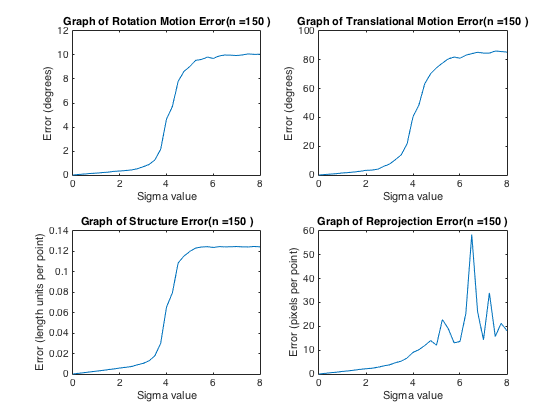
\includegraphics[width=.7\textwidth,keepaspectratio]{experiment_1_error_plots.png}

	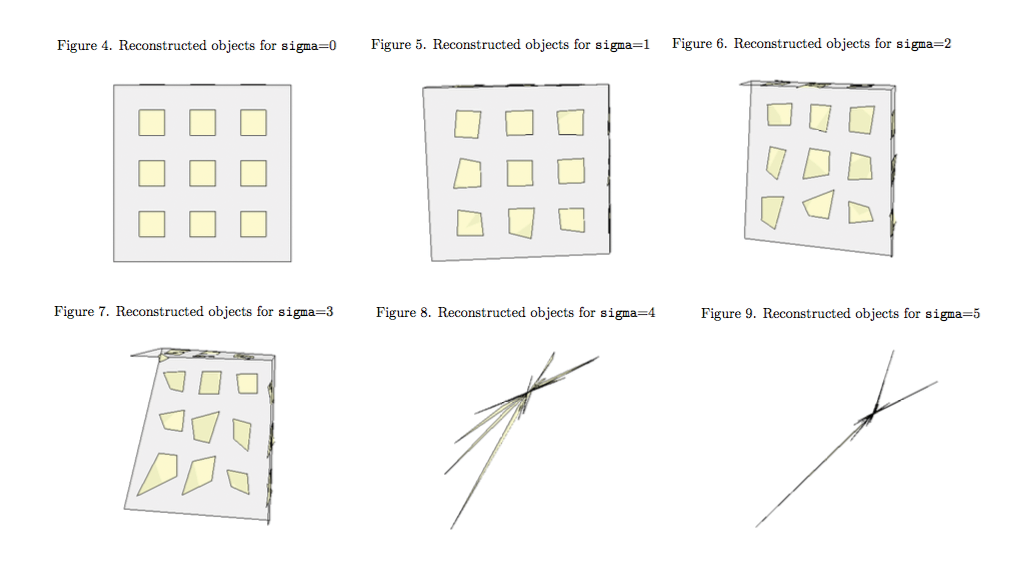
\includegraphics[width=\textwidth,keepaspectratio]{reconstructed_objects.png}
\end{center}


\begin{tabular}{ |p{3cm}|p{3cm}|p{3cm}|p{3cm}|  }
 \hline
 \multicolumn{4}{|c|}{Table 1: Errors for Randomly Generated Image Points for n = 1000} \\
 \hline
 Rotation Error & Translational Error & Structure Error & Reprojection Error\\
 \hline
 127.4189 & 64.2218 & 0.1249 & 4.2279e+04\\
 \hline
\end{tabular}

TODO: graph reprojection error 

% Conclusions

\subsection{Conclusions}

Clearly, there is a severe drop in quality of the reconstructed object after sigma reaches around 3.25, and the reconstructed object for sigma=4 (Figure 8) is completely unrecognizable.

As we can see from the error plots, there is an inflection point around 3.25 where motion error (especially translation error) begins to climb drastically. This is followed immediately by structure error, which also has a similar inflection point. Finally, there is a slight inflection point in reprojection error, which is relatively delayed compared to the other errors (around sigma=4.25).

% TODO: explain why sigmoid (linear until inflection point is because reconstruction fails)

Why is the graph approximately linear before the inflection point? As we increase sigma, the Gaussian noise-generating function gets linearly scaled, making the slight errors increase linearly (on average).

Why is there an inflection point around sigma=3.25? That is the point where there is enough error for catastrophic failure in the reconstructed object such that it becomes unrecognizable. Again, this point exists because 3D reconstruction is an ill-posed problem, where minor errors in input result in massive failures in output. This inflection point is exactly that amount of errors. As obvious in figure 8 and 9, the object is completely unrecognizable after this inflection point.

% TODO: explain why tapers off 

After a certain point, however, the image has enough noise so that it is essentially a random image (one with random values for pixels), uncorrelated with the original object. This is essentially the maximum amount of average error attainable, and is the reason why the error rate tapers off (at around 10 degrees for rotation error, 80 degrees for translation error, and 0.12 unit lengths per point for structural error, according to figures 1-3). To confirm this, we devised the experiment in the section labeled ``Errors for Randomly Generated Image Points for n = 1000'', where we took the average errors for \textit{1000 randomly generated point clouds} after attempted 3D reconstruction. Evidently, the translational and structure error were clearly approximately to the asymptotes of figure 2 and 3 respectively, which showed that at large enough sigma values (approx. 6 and above), the reconstructed figures were \textit{no better than random noise} in terms of correlation with the original object.

% TODO: explain this with data


TODO: why reprojection is only non-sigmoid



TODO: reprojection error changes (0 -- $>$ straight line -- $>$ random points)

The reprojection error plots for different sigma are also insightful in showing the progression of reprojection error as the reconstructed image experiences failure. When sigma is 0, the plot includes all points that are essentially 0-- indicating an almost perfect reconstruction of the reprojected image. However, as sigma gets larger but below the inflection point talked about above, the errors all lie on a straight line-- since the size of the displacements depend roughly \textit{only on distance from the camera} (because of the nature of projecting a 3D object down onto 2D, where farther points seem smaller). Finally, when the sigma reaches the point where catastrophic failure occurs, the displacements become a random cluster around the origin (the reprojected image now no longer has much correlation to the original object). TODO: reference figures



% Things learned

% Problems/ things to learn





\section{Effects of modifying image resolution}

\subsection{Introduction}

\subsection{Data}
\begin{center}
	\begin{center}Figure 10. Error Plots for Resolution of 960x540\end{center}
	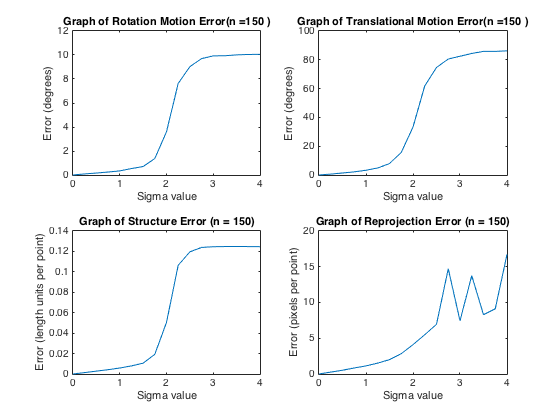
\includegraphics[width=.7\textwidth,keepaspectratio]{960x540_error_plots.png}
	
	\begin{center}Figure 11. Error Plots for Resolution of 1920x1080\end{center}
	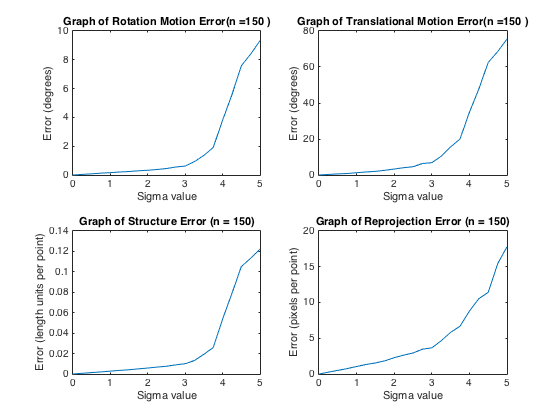
\includegraphics[width=.7\textwidth,keepaspectratio]{1920x1080_error_plots.png}
	
	\begin{center}Figure 12. Error Plots for Resolution of 3840x2160\end{center}
	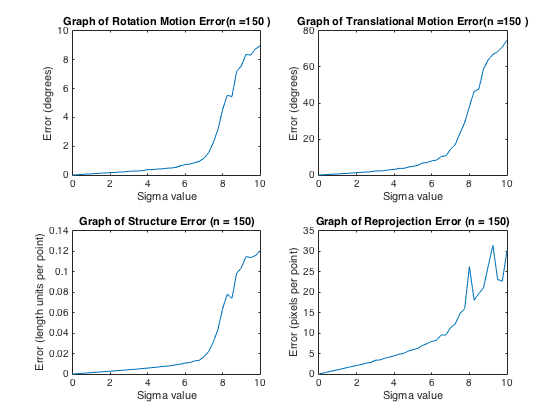
\includegraphics[width=.7\textwidth,keepaspectratio]{3840x2160_error_plots.png}


\end{center}

\subsection{Conclusions}

% TODO: higher res --> lower error (because in pixels)

Clearly, a higher resolution leads to a lower error for fixed sigma. Since sigma is given in pixels, it's obvious that increasing the resolution of the image (i.e. scaling the number of pixels per point) will lead to a lessened effect from the noise-generating function.


% TODO: what relationship is (O(n)), direct scaling

It is interesting to note, however, that the relationship is linear. Observe that the error values for (for example) sigma=1 in a resolution of 960x540 are approximately equal to sigma=2 for resolution 1920x1080 and sigma=4 for resolution 3840x2160. In fact, each plot of a certain resolution is simply the horizontal scaling of the plot of the image half its resolution. 

% TODO: explain why (Gaussian sigma affects both dimensions)

This is because the sigma value scales the randomly generated values in the same number of dimensions as the image (2), which means that an increase of sigma is offset by a proportional increase in both dimensions of resolution (i.e. in an image with double resolution in both dimensions, the equivalent sigma is also double).



\section{Conclusion}



\begin{thebibliography}{99}
\bibitem{hartley}
	Hartley, Richard. ``In defense of the eight-point algorithm.'' Pattern Analysis and Machine Intelligence, IEEE Transactions on 19, no. 6 (1997): 580-593.

\bibitem{chojnacki}
	Chojnacki, Wojciech, and Michael J. Brooks. ``On the consistency of the normalized eight-point algorithm.'' Journal of Mathematical Imaging and Vision 28, no. 1 (2007): 19-27.
\end{thebibliography}


\end{document}